% !TEX TS-program = XeLaTeX
% use the following command:
% all document files must be coded in UTF-8
\documentclass[portuguese]{textolivre}
% build HTML with: make4ht -e build.lua -c textolivre.cfg -x -u article "fn-in,svg,pic-align"

\journalname{Texto Livre}
\thevolume{18}
%\thenumber{1} % old template
\theyear{2025}
\receiveddate{\DTMdisplaydate{2025}{4}{8}{-1}} % YYYY MM DD
\accepteddate{\DTMdisplaydate{2025}{5}{12}{-1}}
\publisheddate{\DTMdisplaydate{2025}{5}{31}{-1}}
\corrauthor{André Luis Antonelli}
\articledoi{10.1590/1983-3652.2025.58530}
%\articleid{NNNN} % if the article ID is not the last 5 numbers of its DOI, provide it using \articleid{} commmand 
% list of available sesscions in the journal: articles, dossier, reports, essays, reviews, interviews, editorial
\articlesessionname{articles}
\runningauthor{Antonelli} 
%\editorname{Leonardo Araújo} % old template
\sectioneditorname{Daniervelin Pereira}
\layouteditorname{Leonado Araújo}

\title{Desafios de grandes modelos de linguagem generativa na reprodução de complexidade textual: um estudo com editoriais jornalísticos}
\othertitle{Challenges for large generative language models in reproducing textual complexity: a study on newspaper editorials}
% if there is a third language title, add here:
%\othertitle{Artikelvorlage zur Einreichung beim Texto Livre Journal}

\author[1]{André Luis Antonelli~\orcid{0000-0002-7896-5465}\thanks{Email: \href{mailto:alantonelli@uem.br}{alantonelli@uem.br}}}
\affil[1]{Universidade Estadual de Maringá, Departamento de Língua Portuguesa, Maringá, PR, Brasil.}

\addbibresource{article.bib}
% use biber instead of bibtex
% $ biber article

% used to create dummy text for the template file
\definecolor{dark-gray}{gray}{0.35} % color used to display dummy texts
\usepackage{lipsum}
\SetLipsumParListSurrounders{\colorlet{oldcolor}{.}\color{dark-gray}}{\color{oldcolor}}

% used here only to provide the XeLaTeX and BibTeX logos
\usepackage{hologo}

% if you use multirows in a table, include the multirow package
\usepackage{multirow}

% provides sidewaysfigure environment
\usepackage{rotating}

% CUSTOM EPIGRAPH - BEGIN 
%%% https://tex.stackexchange.com/questions/193178/specific-epigraph-style
\usepackage{epigraph}
\renewcommand\textflush{flushright}
\makeatletter
\newlength\epitextskip
\pretocmd{\@epitext}{\em}{}{}
\apptocmd{\@epitext}{\em}{}{}
\patchcmd{\epigraph}{\@epitext{#1}\\}{\@epitext{#1}\\[\epitextskip]}{}{}
\makeatother
\setlength\epigraphrule{0pt}
\setlength\epitextskip{0.5ex}
\setlength\epigraphwidth{.7\textwidth}
% CUSTOM EPIGRAPH - END

% to use IPA symbols in unicode add
%\usepackage{fontspec}
%\newfontfamily\ipafont{CMU Serif}
%\newcommand{\ipa}[1]{{\ipafont #1}}
% and in the text you may use the \ipa{...} command passing the symbols in unicode

% LANGUAGE - BEGIN
% ARABIC
% for languages that use special fonts, you must provide the typeface that will be used
% \setotherlanguage{arabic}
% \newfontfamily\arabicfont[Script=Arabic]{Amiri}
% \newfontfamily\arabicfontsf[Script=Arabic]{Amiri}
% \newfontfamily\arabicfonttt[Script=Arabic]{Amiri}
%
% in the article, to add arabic text use: \textlang{arabic}{ ... }
%
% RUSSIAN
% for russian text we also need to define fonts with support for Cyrillic script
% \usepackage{fontspec}
% \setotherlanguage{russian}
% \newfontfamily\cyrillicfont{Times New Roman}
% \newfontfamily\cyrillicfontsf{Times New Roman}[Script=Cyrillic]
% \newfontfamily\cyrillicfonttt{Times New Roman}[Script=Cyrillic]
%
% in the text use \begin{russian} ... \end{russian}
% LANGUAGE - END

% EMOJIS - BEGIN
% to use emoticons in your manuscript
% https://stackoverflow.com/questions/190145/how-to-insert-emoticons-in-latex/57076064
% using font Symbola, which has full support
% the font may be downloaded at:
% https://dn-works.com/ufas/
% add to preamble:
% \newfontfamily\Symbola{Symbola}
% in the text use:
% {\Symbola}
% EMOJIS - END

% LABEL REFERENCE TO DESCRIPTIVE LIST - BEGIN
% reference itens in a descriptive list using their labels instead of numbers
% insert the code below in the preambule:
%\makeatletter
%\let\orgdescriptionlabel\descriptionlabel
%\renewcommand*{\descriptionlabel}[1]{%
%  \let\orglabel\label
%  \let\label\@gobble
%  \phantomsection
%  \edef\@currentlabel{#1\unskip}%
%  \let\label\orglabel
%  \orgdescriptionlabel{#1}%
%}
%\makeatother
%
% in your document, use as illustraded here:
%\begin{description}
%  \item[first\label{itm1}] this is only an example;
%  % ...  add more items
%\end{description}
% LABEL REFERENCE TO DESCRIPTIVE LIST - END


% add line numbers for submission
%\usepackage{lineno}
%\linenumbers

\usepackage{amsmath}
\usepackage{enumitem}

\begin{document}
\maketitle

\begin{polyabstract}
\begin{abstract}
Este artigo avalia a \emph{performance} do modelo de linguagem generativa \emph{Sabiá-3} na tarefa de reproduzir aspectos de complexidade textual do gênero discursivo editorial, usando como ponto de referência editoriais produzidos por humanos.
Para essa tarefa, utilizamos métricas da ferramenta computacional NILC-Metrix.
Nossos resultados revelaram diferenças em quatro das cinco métricas analisadas.
Os textos humanos demonstraram maior complexidade nas medidas ``proporção de types em relação à quantidade de tokens'' e ``entropia cruzada''.
Argumentamos que esse resultado pode estar vinculado, por exemplo, à capacidade humana de selecionar palavras ou realizar combinações lexicais sem a limitação de parâmetros probabilísticos.
Já os textos gerados pelo modelo \emph{Sabiá-3} apresentaram maior complexidade nas métricas ``sílabas por palavra'' e ``orações subordinadas'', possivelmente devido ao fato, entre outros aspectos, de que ferramentas do tipo não sofrem restrições de processamento cognitivo.
A única métrica sem diferença estatística significativa foi ``conjunções difíceis''.
Atribuímos esse resultado à natureza fechada dessa classe gramatical, que limitaria variações.
O estudo reforça a importância de se considerar múltiplas dimensões da complexidade textual ao avaliar a produção de grandes modelos de linguagem generativa, especialmente quando se trata de gêneros que exigem domínio linguístico refinado, tais como o editorial.

\keywords{Modelos de linguagem generativa \sep Complexidade textual \sep Gêneros discursivos \sep Inteligência artificial e linguagem \sep Análise comparativa humano-IA}
\end{abstract}

\begin{english}
\begin{abstract}
This article evaluates the performance of the generative language model \emph{Sabiá-3} in the task of reproducing aspects of textual complexity characteristic of the editorial discourse genre, using human-produced editorials as a reference point.
For this task, we employed metrics from the computational tool NILC-Metrix.
Our results revealed differences in four out of the five analyzed metrics. Human texts showed greater complexity in the measures of ``type-token ratio'' and ``cross-entropy''.
We argue that this outcome may be linked, for instance, to the human ability to select words or form lexical combinations without the constraints of probabilistic parameters.
In contrast, the texts generated by the \emph{Sabiá-3} model displayed higher complexity in the ``syllables per word'' and ``subordinate clauses'' metrics, possibly due, among other factors, to the fact that such tools do not face cognitive processing limitations.
The only metric without a statistically significant difference was ``hard conjunctions''.
We attribute this result to the closed-class nature of this grammatical category, which tends to limit variation.
This study reinforces the importance of considering multiple dimensions of textual complexity when evaluating the output of large generative language models, especially in genres that require refined linguistic control, such as the editorial.

\keywords{Generative language models \sep Textual complexity \sep Discourse genres \sep Artificial intelligence and language \sep Human-AI comparative analysis}
\end{abstract}
\end{english}
% if there is another abstract, insert it here using the same scheme
\end{polyabstract}

\section{Introdução}\label{sec-intro}
Grandes modelos de linguagem generativa (LLMs, na sigla em inglês) têm desempenhado um papel crescente na produção automatizada de textos \cite{Reisenbichler2022, Franceschelli2024, Naik2024}, sendo empregados em uma ampla variedade de aplicações, desde a redação de conteúdos jornalísticos até a assistência na escrita acadêmica e técnica.
Deixando de lado a questão ética, que envolve discussões, entre outros aspectos, sobre autoria, autenticidade e impactos no mercado de trabalho, o fato é que essas ferramentas, treinadas a partir de enormes \emph{corpora}, têm demonstrado notável habilidade na geração de textos em diversos domínios.
No entanto, apesar de tais avanços, muitos pontos ainda precisam ser melhor explorados.  Um deles diz respeito à capacidade de tais modelos de mimetizar com precisão aspectos relacionados à complexidade textual de gêneros discursivos específicos.

Como já bem estabelecido na literatura especializada, cada gênero do discurso apresenta convenções próprias, que moldam a organização da informação, a escolha lexical, a estrutura sintática e os recursos argumentativos empregados na construção dos enunciados linguísticos \cite{Bakhtin1997}.
A combinação dessas propriedades impacta naquilo que podemos chamar de nível de complexidade de um texto.
De acordo com  \textcite{Frantz2015}, complexidade textual refere-se ao grau de sofisticação e desafio que um texto coloca ao leitor, podendo ser analisada com base em fatores linguísticos, cognitivos e discursivos.
Ela é frequentemente avaliada por meio da diversidade lexical, do grau de estruturação sintática, da coesão e de medidas de leiturabilidade.
Essa natureza multifacetada da complexidade textual é um elemento importante na diferenciação dos gêneros discursivos entre si.
Por exemplo, em termos de tipologia textual, uma charge pode ser tão opinativa quanto um editorial de jornal, ainda que sejam gêneros do discurso distintos.
No entanto, não há dúvida de que estamos diante de manifestações linguísticas que mobilizam diferentes níveis de complexidade, seja na forma de estrutura organizacional, seja na forma de disposição dos argumentos ou mesmo no grau de diversidade lexical, para nomear apenas algumas distinções.
Isso mostra que a relação entre gêneros discursivos e complexidade textual é intrínseca, pois cada gênero, ao se adaptar às convenções que lhe são impostas, apresenta níveis de complexidade específicos.
Assim, quando pensamos em produção automatizada de textos por LLMs, a questão que se coloca é saber não apenas o nível de proficiência dessas ferramentas em produzir conteúdo que seja coerente e adequado às normas linguísticas, mas também a capacidade de se adaptar ao nível de complexidade textual exigida pelo gênero do discurso a ser gerado.

Como contribuição a esse debate, neste artigo avaliaremos a \emph{performance} de um modelo de linguagem generativa na tarefa de reproduzir aspectos de complexidade textual do gênero discursivo editorial, usando como ponto de referência editoriais produzidos por humanos.
Para essa tarefa, empregaremos uma série de métricas quantitativas de complexidade linguística, o que possibilitará uma avaliação multidimensional do fenômeno.
Esperamos, com isso, fornecer uma análise objetiva das capacidades e limitações de LLMs na reprodução de propriedades de complexidade textual intrínsecas à configuração discursiva de qualquer produção verbal.

O artigo está organizado da seguinte maneira.
A \Cref{sec-fundamentação} apresenta a fundamentação teórica a ser explorada no trabalho.
Na \Cref{sec-metodologia}, detalhamos os procedimentos metodológicos adotados.
A \Cref{sec-resultados} é dedicada à apresentação dos resultados, que serão analisados na \Cref{sec-discussão}.
Por fim, na \Cref{sec-conclusão}, apresentamos as considerações finais.

\section{Fundamentação teórica}\label{sec-fundamentação}

\subsection{Gêneros textuais e o editorial jornalístico}\label{sec-gêneros}
Os gêneros textuais são categorias que agrupam textos com características linguísticas, discursivas e funcionais semelhantes, moldadas por contextos sociocomunicativos específicos \cite{Bakhtin1997}.
Eles surgem a partir das necessidades de comunicação em diferentes esferas da atividade humana.
Cada gênero é caracterizado por uma estrutura e uma função social próprias, que orientam tanto a produção quanto a interpretação dos textos.

Dentro da esfera de gêneros jornalísticos que circulam socialmente, o editorial é um exemplo emblemático de texto opinativo, cuja função principal é expressar a posição institucional de um veículo de comunicação sobre temas de relevância pública.
Os editoriais são marcados por uma estrutura clássica que inclui uma introdução, na qual o tema é contextualizado; um desenvolvimento, que apresenta argumentos fundamentando a tese a ser defendida; e uma conclusão, que reforça a posição assumida no texto \cite{Vieira2009}.
Linguisticamente, esse gênero se destaca pelo emprego de um estilo formal, que se caracteriza pelo uso de vocabulário e estruturas gramaticais típicas da norma urbana culta.
Além disso, os editoriais se caracterizam pelo uso de estratégias discursivas que buscam persuadir o leitor, como o emprego de evidências estatísticas, referências a autoridades e apelos emocionais.
Essas características fazem desse gênero textual uma estrutura sofisticada, que exige do autor não apenas domínio linguístico, mas também profundidade argumentativa e sensibilidade ao contexto sociopolítico.

A complexidade dos editoriais também se reflete em sua função social.
Como textos opinativos, desempenham um papel crucial na formação da opinião pública, procurando influenciar a maneira como os leitores percebem e interpretam eventos e questões relevantes do cotidiano.
Essa função exige que os editoriais sejam ao mesmo tempo claros e persuasivos, equilibrando a necessidade de transmitir informações de maneira acessível com a de apresentar argumentos convincentes e bem fundamentados.
Esse conjunto de propriedades de natureza gramatical, argumentativa e social tornam o editorial um gênero particularmente interessante para análises comparativas entre humanos e inteligência artificial (IA), uma vez que estamos diante de uma manifestação linguística com diferentes camadas, todas elas contribuindo para o grau de complexidade textual do material produzido.

\subsection{Modelos de linguagem generativa}\label{sec-modelos}
Grandes modelos de linguagem generativa, como, por exemplo, os da família GPT (\emph{Generative Pre-trained Transformer}) e Llama, têm reconfigurado o campo de estudos sobre processamento de linguagem natural.
Esses modelos são baseados na arquitetura \emph{Transformer}, proposta por \textcite{Vaswani2018}, que utiliza mecanismos de atenção (\emph{attention mechanisms}) para processar e gerar textos.

Historicamente, os modelos de linguagem evoluíram de abordagens estatísticas simples, como n-gramas, para sistemas capazes de lidar com tarefas complexas, como tradução automática, sumarização e geração de texto.
Os LLMs modernos são treinados em \emph{corpora} de grande escala, que incluem materiais de diversos gêneros e domínios, o que lhes permite gerar textos em uma ampla variedade de estilos e contextos.

Uma característica central dessas ferramentas de IA é justamente a capacidade de produzir textos de forma contextualizada, baseada na análise de padrões sintáticos, semânticos e discursivos aprendidos durante o treinamento.
De acordo com \textcite{Radford2019}, essa capacidade é possibilitada pelo mecanismo de atenção, que permite ao modelo atribuir pesos distintos a diferentes partes do prompt de entrada, resultando em respostas mais coesas e pertinentes.
Tal mecanismo confere aos modelos uma flexibilidade que lhes permite adaptar-se, por exemplo, a diferentes gêneros textuais.
Além disso, estudos como o de \textcite{Touvron2023} demonstram que esses grandes modelos de linguagem generativa conseguem alcançar um nível avançado de compreensão textual, respondendo adequadamente às tarefas solicitadas.
 
\subsection{Métricas de complexidade textual}\label{sec-métricas}
A medição da complexidade textual é uma tarefa multifacetada por excelência, abrangendo dimensões variadas.
A depender de como o conceito de complexidade é desenvolvido, ele pode incluir desde elementos estritamente linguísticos, como o grau de sofisticação do vocabulário empregado, até fatores predominantemente cognitivos, como a necessidade de o leitor integrar as novas informações apresentadas com seu repertório de conhecimentos prévios \cite{Frantz2015}.

Diversas métricas e ferramentas já foram desenvolvidas para mensurar a complexidade textual.
Entre as abordagens mais utilizadas estão métricas de diversidade lexical, como a razão type-token (TTR), medidas de complexidade sintática, como o comprimento médio das sentenças, e indicadores de coesão e coerência textual.
Uma das vantagens dessas métricas é o fato de permitirem uma avaliação quantitativa da complexidade, conferindo um nível adicional de objetividade às análises.

Entretanto, tais métricas apresentam limitações se aplicadas de maneira isolada.
Um argumento interessante nesse sentido é dado por \textcite{Mcnamara2002}.
Comparando os exemplos (\ref{ex1}) e (\ref{ex2}), os autores mostram que o primeiro deles apresenta um nível de coesão mais baixo, pois não há nenhuma indicação linguística que aponte a relação de causa entre as duas sentenças.
O resultado desse menor nível de coesão é que, diante de um exemplo como (\ref{ex1}), o leitor teria um desafio maior para estabelecer a relação de causa, já que isto poderia ser inferido unicamente a partir da condição de adjacência entre as duas sentenças do enunciado
Em outras palavras, unicamente por essa métrica, o exemplo (\ref{ex1}) seria considerado mais complexo, pois impõe um nível maior de interpretação.
Porém, um índice de complexidade que levasse em consideração apenas o parâmetro sintático de tamanho da sentença apontaria que o exemplo (\ref{ex1}) é mais simples do que o exemplo (\ref{ex2}), pois se trata de um enunciado menor.
O que esses dados mostram, na análise dos autores, é que a complexidade textual deve ser medida de maneira mais ampla, por meio da aplicação de diferentes métricas.

\begin{enumerate}[resume=exlist]
\item One part of the cloud develops a downdraft. Rain begins to fall\footnote{``Uma parte da nuvem desenvolve uma corrente de ar descendente. A chuva começa a cair'' (tradução nossa).}.\label{ex1}
\item One part of the cloud develops a downdraft, which causes rain to fall\footnote{``Uma parte da nuvem desenvolve uma corrente de ar descendente, o que faz com que a chuva comece a cair'' (tradução nossa).}.\label{ex2}
\end{enumerate}

No contexto do português brasileiro, a ferramenta NILC-Metrix\footnote{\url{http://fw.nilc.icmc.usp.br:23380/nilcmetrix}.} destaca-se como, talvez, o mais importante recurso para análise de complexidade textual.
Desenvolvido pelo Núcleo Interinstitucional de Linguística Computacional (NILC)\footnote{\url{https://sites.google.com/view/nilc-usp/}.}, o NILC-Metrix integra 200 métricas linguísticas, cobrindo áreas como complexidade sintática, diversidade lexical, uso de conectivos e coesão textual, entre outros aspectos \cite{Leal2024}.
Esse conjunto de métricas oferece uma visão multidimensional da estrutura textual, permitindo a análise não apenas de características superficiais, como comprimento de palavras e sentenças, mas também de aspectos mais profundos, como a organização discursiva e a progressão temática.
E é justamente por essa capacidade de analisar múltiplas dimensões da complexidade textual de forma integrada que o NILC-Metrix é especialmente útil para avaliar a performance de LLMs na reprodução de um gênero do discurso tão complexo como o editorial.

\section{Metodologia}\label{sec-metodologia}

\subsection{Coleta de dados}\label{sec-coleta}
Para a investigação que nos propusemos a fazer aqui, coletamos cinquenta editoriais do jornal \emph{Folha de São Paulo} (FSP)\footnote{\url{https://www.folha.uol.com.br/}.}, publicados entre os dias 27 de setembro e 21 de outubro de 2024.
Esses textos foram selecionados para representarem a amostra de editoriais produzidos por humanos
No caso específico dos editoriais da FSP, são textos escritos por uma equipe de editorialistas e representam o ponto de vista da empresa sobre os assuntos discutidos\footnote{\url{https://www1.folha.uol.com.br/tv/2022/07/folha-explica-a-diferenca-entre-os-tipos-de-texto-que-voce-le-no-jornal.shtml}.}.

Paralelamente, foram produzidos cinquenta textos utilizando o modelo de inteligência artificial generativa \emph{Sabiá-3}, desenvolvido pela empresa brasileira Maritaca AI\footnote{\url{https://www.maritaca.ai/}.}.
Trata-se de um modelo treinado com um corpus de dados disponíveis até meados de 2023.
O \emph{Sabiá-3} é baseado na arquitetura \emph{Transformers}, no entanto a configuração exata, incluindo o número de parâmetros, é uma informação não disponibilizada pela empresa.
Apesar dessa não publicização, o que pode ser visto como uma propriedade desfavorável, uma vantagem da ferramenta nacional em relação a outros modelos é o fato de ter sido treinada exclusivamente com dados em língua portuguesa, o que a torna particularmente adequada para a geração de textos nessa língua.
Um relatório técnico sobre esse LLM é apresentado em \textcite{Abonizio2025}.

Os textos gerados pela IA foram produzidos com base no seguinte prompt: ``Escreva um editorial de jornal, com aproximadamente 425 palavras\footnote{Essa é quantidade média de palavras dos editoriais da FSP.}, sobre o seguinte assunto:'', seguido do título e subtítulo de um editorial real da FSP.
Para cada editorial produzido pelo LLM, utilizou-se o título e o subtítulo de um dos editoriais da amostra humana.
Como o \emph{Sabiá-3} foi treinado com material disponível até meados de 2023, essa abordagem garantiu que o modelo não tivesse acesso aos editoriais humanos que utilizamos, evitando desse modo eventuais plágios.
Além disso, como os editoriais da FSP e aqueles gerados pela IA abordam a mesma temática, isso minimiza eventuais discrepâncias que pudessem surgir entre as amostras por conta de diferenças temáticas.

\subsection{Ferramenta de análise e métricas selecionadas}\label{sec-ferramenta}
Para avaliar a complexidade textual dos editoriais, utilizamos o NILC-Metrix, já apresentado na \Cref{sec-métricas}.
Tendo em vista as restrições de espaço para se analisar em um único artigo os resultados de todas as métricas, escolhemos cinco delas, apresentadas a seguir.

\begin{enumerate}[label=\Roman*.]
    \item \textbf{Sílabas por palavra.} Essa métrica calcula o número médio de sílabas por palavras de conteúdo no texto.
São consideradas palavras de conteúdo os itens vocabulares de quatro classes gramaticais: substantivos, verbos, adjetivos e advérbios. Assume-se que um número maior de sílabas por palavras corresponde a um grau de complexidade maior.
    \item \textbf{Proporção de types em relação à quantidade de tokens.} Trata-se de uma métrica que computa a proporção de palavras sem repetições (types) em relação ao total de palavras com repetições (tokens). Cada flexão é tratada como um type diferente. Na documentação oficial do NILC-Metrix, considera-se que a complexidade de um texto é proporcional ao valor dessa métrica, isto é, valores maiores correspondem a textos mais complexos.
    \item \textbf{Orações subordinadas.} Essa métrica calcula a proporção de orações subordinadas pela quantidade de orações do texto. Assume-se que orações dependentes são estruturas mais complexas, demandando um maior esforço de processamento. Assim, quanto maior o resultado dessa métrica, maior a complexidade textual.
    \item \textbf{Conjunções difíceis.} Trata-se de uma métrica que computa a proporção de conjunções difíceis em relação a todas as palavras do texto. A interpretação da métrica é que quanto maior o resultado obtido, maior a complexidade textual. Os itens lexicais que fazem parte dessa categoria são:
    todavia, eis, a fim de, ao passo que, para que, conforme, tais, ou seja, contudo, bem como, logo, à medida que, entretanto, desde que, mesmo que, ainda que, de acordo com, uma vez que, por sua vez, sobretudo, até, ainda, caso, no entanto, nem, quanto, já, como, já que, outrossim, mas também, como também, não só, mas ainda, tampouco, senão também, bem assim, ademais, antes, não obstante, sem embargo, ao passo que, de outra forma, em todo caso, aliás, de outro modo, por conseguinte, em consequência de, por consequência, consequentemente, conseguintemente, isso posto, pelo que, de modo que, de maneira que, de forma que, em vista disso, por onde, porquanto, posto que, isto é, ademais, senão, dado que, visto como, vez que, de vez que, pois que, agora, na medida em que, sendo que, como que, como quer que, eis que, sendo assim, tal qual, ao invés de, conquanto, por muito que, visto que, uma vez que, quanto mais, quanto menos, se bem que, apesar de que, suposto que, ainda quando, quando mesmo, a despeito de, conquanto que, sem embargo de que, por outro lado, em contrapartida, sem embargo, muito embora, inclusive se, por mais que, por menos que, por pouco que, contanto que, salvo se, com tal que, caso que, consoante, tal que, de forma que, à proporção que, ao passo que, mal, tão logo, entretanto, sob esse aspecto, sob esse prisma, sob esse ponto de vista, sob esse enfoque, embora, portanto, além disso\footnote{Essa lista foi definida por um linguista da antiga plataforma Guten Educação, agora denominada Árvore Atualidades (\url{https://www.arvore.com.br/}). Na documentação oficial do NILC-Metrix, nenhuma informação adicional de autoria e critérios de classificação é apresentada.}.
    \item \textbf{Entropia cruzada.} Essa métrica avalia o grau de ``surpresa'' de um modelo de linguagem ao processar uma sentença, calculando a média do valor de entropia cruzada das sentenças do texto. Para calcular essa medida, o NILC-Metrix utiliza um modelo estatístico de trigramas com suavização Kneser-Ney modificada, gerado pela ferramenta KenLM (\url{https://github.com/kpu/kenlm}). Os valores obtidos podem variar de 0 a 1. Um índice maior de entropia cruzada corresponde a uma maior complexidade das palavras em relação ao modelo de língua estatístico treinado, isto é, valores maiores representam um nível maior de combinações não usuais de palavras.
\end{enumerate}




\section{Resultados}\label{sec-resultados}
Na \Cref{tbl-tabela-01}, apresentamos a média geral para cada uma das cinco métricas escolhidas no estudo\footnote{Os resultados obtidos foram submetidos a uma análise estatística com o software R 4.2.2 \cite{R2021}.}.

\begin{table}[htpb]
\centering
\begin{threeparttable}
\caption{Média dos valores das métricas escolhidas para as amostras de editoriais produzidos por humanos e editoriais gerados pelo modelo \emph{Sabiá-3}.}
\label{tbl-tabela-01}
\begin{tabular}{lcc}
\toprule 
Métrica & Humanos & IA \\ 
\midrule
  Sílabas por palavra & 2.931442 & 3.247690 \\
  Proporção de types em relação à quantidade de tokens & 0.7845508 & 0.7373788 \\
  Orações subordinadas & 0.5021336 & 0.5897614 \\ 
  Conjunções difíceis & 0.0234116 & 0.0211284 \\
  Entropia cruzada & 0.5843956 & 0.4559052 \\
\bottomrule
\end{tabular}
\source{Elaboração própria.}
\end{threeparttable}
\end{table}

Para verificar se as diferenças de média entre a amostra de editoriais humanos e a amostra de editoriais gerados por IA são estatisticamente significativas, aplicamos o teste $t$ para duas amostras independentes.
Esse teste tem o objetivo de comparar o efeito de uma mesma variável em duas populações independentes e distribuídas identicamente.
A estatística do teste $t$ é dada por
\begin{equation}
  t = \frac{\bar{X}_1 - \bar{X}_2}{\sqrt{s_p^2 \left( \frac{1}{n_1} + \frac{1}{n_2} \right) }} ,
  \label{eq-teste_t}
\end{equation}

onde:
\begin{itemize}
\item \( \bar{X}_1, \bar{X}_2 \) são as médias amostrais dos dois grupos;
\item \( s_1^2, s_2^2 \) são as variâncias amostrais;
\item \( n_1, n_2 \) são os tamanhos das amostras;
\item \( s_p^2 \) é a variância combinada.
\end{itemize}

O teste $t$ para duas amostras independentes testa as seguintes hipóteses:
\begin{itemize}
\item Hipótese nula (H$_0$): as médias das duas populações são iguais, ou seja, eventuais diferenças não são estatisticamente significativas;
\item Hipótese alternativa (H$_1$): as médias das populações são diferentes, ou seja, diferenças atestadas são estatisticamente significativas.
\end{itemize}

No nosso caso, H$_0$ assume que as diferenças de média entre as duas amostras para cada métrica de complexidade textual não são estatisticamente significativas se o nível de significância (valor de $p$) associado ao índice de $t$ for maior que 0.05, o que equivale dizer que as diferenças de média não são afetadas pela variável tipo de produtor (humanos \emph{versus} IA).
Já H$_1$ postula que as diferenças de média entre as duas amostras são estatisticamente significativas (com o valor de $p \leq 0.05$), ou seja, a variável tipo de produtor afeta as diferenças de média.
Os resultados de aplicação do teste $t$ são apresentados na \Cref{tbl-tabela-02}.

\begin{table}[htpb]
\centering
\begin{threeparttable}
\caption{Valores do teste $t$ para as métricas escolhidas e respectivos valores de $p$.}
\label{tbl-tabela-02}
\begin{tabular}{lcc}
\toprule 
Métrica & valor de $t$ & valor de $p$ \\ 
\midrule
  Sílabas por palavra & -12.134 & <2.2e-16 \\
  Proporção de types em relação à quantidade de tokens & 12.554 & <2.2e-16 \\
  Orações subordinadas & -6.5845 & 2.276e-09 \\ 
  Conjunções difíceis & 1.3349 & 0.185 \\
  Entropia cruzada & 20.223 & <2.2e-16 \\
\bottomrule
\end{tabular}
\source{Elaboração própria.}
\end{threeparttable}
\end{table}

Como mostram os resultados da \Cref{tbl-tabela-02}, ``conjunções difíceis'' é a única métrica que não apresenta uma diferença de média estatisticamente significativa.
Todas as outras apresentam valores de $t$ associados a níveis de significância abaixo de 0.05, o que nos leva a assumir que, no caso dessas quatro métricas, as diferenças de média são estatisticamente significativas, implicando que há efeito da variável tipo de produtor sobre o resultado da média.

Esses resultados são reforçados quando olhamos para os diagramas de caixa na \Cref{fig-img-01}.
Ali vemos que, apenas na métrica ``conjunções difíceis'', o intervalo interquartil das duas amostras apresenta uma considerável sobreposição, o que aponta para uma dispersão dos dados centrais mais próxima entre os dois conjuntos.
Isso vai ao encontro do resultado de que a diferença de média entre textos humanos e textos gerados por IA na métrica ``conjunções difíceis'' não é estatisticamente significativa.
Nas demais métricas, o que se vê é uma clara falta de alinhamento da dispersão dos dados centrais, o que corrobora o resultado já apresentado de que, para tais métricas, as diferenças de média entre as duas amostras são estatisticamente significativas.

\begin{figure}[htbp]
\centering
\begin{minipage}{1\textwidth}
\centering
  \includegraphics[width=.5\linewidth, height=14cm, angle=270]{figura_01.ps}
 \caption{Medidas de dispersão e tendência central para as métricas ``sílabas por palavra'' (A), ``proporção de types em relação à quantidade de tokens'' (B), ``orações subordinadas'' (C), ``conjunções difíceis'' (D) e ``entropia cruzada'' (E).}
 \label{fig-img-01}
 \source{Elaboração própria.}
\end{minipage}
\end{figure}

\section{Discussão}\label{sec-discussão}

\subsection{Métricas com maior complexidade na amostra humana}\label{sec-humanos}
Iniciamos a discussão dos resultados comentando as duas métricas em que a amostra de editoriais produzidos por humanos apresentou índices de média, com diferenças estatisticamente significativas, superiores aos valores obtidos pela amostra de textos gerados pelo modelo \emph{Sabiá-3}.
Essas duas métricas, como apontado na \Cref{sec-resultados}, são ``proporção de types em relação à quantidade de tokens'' e ``entropia cruzada''.
Em ambas, valores maiores correspondem a índices mais elevados de complexidade textual, o que nos permite dizer que, nesses quesitos, os textos humanos se mostram mais complexos.

Um primeiro ponto a ser destacado para explicar essa maior complexidade dos editoriais humanos diz respeito à métrica ``proporção de types em relação à quantidade de tokens''.
A média maior nessa medida sugere um uso mais diversificado do léxico.
No caso dos editoriais da FSP, essa diversidade mais elevada pode estar vinculada à criatividade típica da escrita humana.
Enquanto LLMs operam com distribuições estatísticas aprendidas a partir de \emph{corpora}, escritores humanos selecionam palavras não apenas com base em probabilidades, mas também motivados por nuances semânticas, estilísticas e pragmáticas \cite{Piantadosi2014}.
Essa flexibilidade permite maior inovação lexical, incluindo o uso de palavras menos frequentes ou combinações inusitadas, elevando a proporção de types.
Já as ferramentas de IA priorizam tokens mais comuns para garantir coerência, o que acaba por reduzir a diversidade lexical \cite{Holtzman2020}.

Outro aspecto da relação type/token é que LLMs fazem uso de padrões repetitivos como estratégia para minimizar erros ou incoerências.
Esse comportamento, conhecido como ``degeneração'' (\emph{degeneracy}), é documentado, por exemplo, em \textcite{Welleck2019}, que observam a tendência de modelos generativos repetirem estruturas ou palavras para manter a fluência superficial.
Em contraste, particularmente em contextos formais, escritores humanos monitoram ativamente a redundância, ajustando o texto para evitar repetições desnecessárias --- um processo vinculado à ``teoria da monitoração'' \cite{Levelt1989}.
Assim, a menor proporção de types/tokens nos textos gerados por IA pode refletir essa busca conservadora dos grandes modelos de linguagem generativa por segurança estatística.

Outro ponto a ser detacado em relação a essa métrica tem a ver com o fato de que, como mencionado anteriormente, o NILC-Metrix considera flexões como types distintos, o que pode apontar para uma certa incapacidade dos LLMs em utilizar variações morfológicas sutis.
Por exemplo, em textos escritos formais, ainda é usual em produções humanas a presença de formas verbais mais raras na fala, como flexões do modo subjuntivo \cite{Almeida2010}.
Já em relação a grandes modelos de linguagem generativa, \textcite{Gulordava2018} demonstram que tais ferramentas apresentam uma maior dificuldade em generalizar padrões morfológicos complexos, especialmente em línguas com alta carga flexional, como é o caso do português.
Essa limitação poderia reduzir a diversidade de types nos textos gerados.

Ainda em relação à proporção types/tokens, cabe dizer que textos humanos são moldados por contextos situacionais e objetivos comunicativos específicos.
Editoriais, em particular, exigem adaptação a audiências, tons e finalidades --- o que incentiva a variação lexical \cite{Biber2009}.
Modelos de linguagem generativa, por outro lado, carecem de intencionalidade genuína.
Sua produção é orientada por prompts, o que pode levar a um repertório lexical mais estático.

No que diz respeito à métrica ``entropia cruzada'', o maior nível de complexidade dos textos humanos nesse quesito também se explica nas mesmas linhas da questão da diversidade lexical explorada para a métrica anterior.
Podemos retomar, por exemplo, o ponto de que LLMs priorizam combinações de palavras mais prováveis, alinhadas aos padrões estatísticos dominantes em seus dados de treinamento, o que reduz a ``surpresa'' medida pela entropia cruzada.
Já textos humanos, como refletem escolhas individuais do autor, influências estilísticas e adpatações contextuais, podem apresentar mais combinações idiossincráticas, consequentemente aumentando o grau de entropia cruzada.

\subsection{Métricas com maior complexidade na amostra automatizada}\label{sec-ia}
Passemos agora às duas métricas em que os textos gerados pelo modelo \emph{Sabiá-3} apresentam uma média maior em relação ao conjunto de editoriais da FSP, a saber, ``sílabas por palavra'' e ``orações subordinadas''.
Nessas métricas, como nas duas anteriores discutidas, vimos que as diferenças são estatisticamente significativas.
Aqui também valores maiores indicam um maior nível de complexidade.
Um primeiro aspecto explicando essa diferença pode estar relacionado a questões de processamento linguístico.
\textcite{Gibson2000} apresenta evidências de que a produção humana de linguagem é limitada por restrições de memória operacional.
Por exemplo, esse autor mostra que o aumento de orações relativas tende a aumentar a dificuldade de compreensão, como ilustrado nos exemplos de (3) a (5).

\begin{enumerate}[resume=exlist]
\item The reporter disliked the editor.\label{ex3}
\item The reporter [\textsubscript{S} who the senator attacked] disliked the editor.\label{ex4}
\item *The reporter [\textsubscript{S} who the senator [\textsubscript{S} who John met] attacked] disliked the editor.\label{ex5}
\end{enumerate}

Em (\ref{ex3}), temos uma oração simples com nenhum material interveniente entre o sujeito \emph{the reporter} e o verbo com o qual ele está associado, \emph{disliked}.
Em (\ref{ex2}), é encaixada uma oração relativa entre o sintagma nominal \emph{the reporter} e o verbo \emph{disliked}.
Em (\ref{ex3}), é colocada uma oração relativa entre o sujeito e o verbo da primeira oração encaixada (\emph{the senator} e \emph{attacked}).
De acordo com o autor, essa última sentença é tão complexa que, para a maioria dos falantes nativos do inglês, ela apresenta uma alta dificuldade de processamento\footnote{Em português, as respectivas traduções para os enunciados de (\ref{ex3}) a (\ref{ex5}) recebem juízos de gramaticalidade equivalentes, sugerindo não se tratar de uma restrição específica do inglês, mas sim de algo mais geral em termos de processamento cognitivo.
  \begin{enumerate}[label=\roman*.]
  \item O repórter não gostava do editor.
  \item O repórter [\textsubscript{S} que o senador atacou] não gostava do editor.
  \item *O repórter [\textsubscript{S} que o senador [\textsubscript{S} que o João encontrou] atacou] não gostava do editor.
  \end{enumerate}}.
Aplicando esse fato à nossa discussão, podemos dizer que o uso excessivo de palavras mais longas ou de orações subordinadas pode sobrecarregar o leitor, o que levaria escritores mais experientes a moderar a sua frequência.
Já os modelos de IA, desprovidos de tais limitações cognitivas, podem gerar estruturas gramaticais densas (sejam elas de natureza fonológica, morfoloógica ou sintática) sem avaliar seu impacto na compreensão.
Isso explicaria por quê o \emph{Sabiá-3} apresenta uma média maior de sílabas por palavras de conteúdo e também de orações subordinadas, quando comparado com a amostra de editoriais humanos.

Especificamente em relação à métrica ``orações subordinadas'', é importante destacar que estruturas encaixadas seguem padrões sintáticos relativamente previsíveis (isto é, são construções sintáticas introduzidas por um conjunto fechado de conjunções, tais como ``que'', ``quando'', ``embora''), o que, por hipótese, facilita sua geração automática.
LLMs podem recorrer a essas estruturas como ``atalhos'' para estender o texto de forma coerente, mesmo quando a subordinação não acrescenta informação relevante.
Consequentemente, essa eventual estratégia de LLMs pode resultar em textos com mais sentenças encaixadas, quando comparados com produções similares realizadas por humanos.

\subsection{Similaridade de complexidade nas duas amostras}\label{sec-similaridade}
Por fim, discutimos  a métrica ``conjunções difíceis'', para a qual não encontramos diferença de média estatisticamente significativa entre as duas amostras.
Em termos quantitativos, isso nos permite dizer que, nessa métrica, as duas amostras apresentam comportamento similar no que diz respeito à complexidade textual.
Ao contrário do que fizemos anteriormente, o ponto agora é saber por que ocorre essa semelhança.
Um aspecto que nos parece importante é a natureza gramatical dos itens lexicais avaliados nessa métrica.
A classe das conjunções é, em termos morfossintáticos, de natureza fechada, já que abriga essencialmente elementos funcionais.
Isso pode ter um impacto no grau de diversidade de uso desses elementos, pois, diferentemente de classes abertas, como substantivos e verbos, as conjunções não permitem uma expansão ilimitada de seu repertório lexical, o que restringe a margem para variação estilística ou criativa, reduzindo o espectro de possíveis diferenças entre produção humana e automatizada.

Uma forma de testar essa hipótese é comparar o comportamento das duas amostras em uma métrica que avalie itens lexicais de alguma classe aberta.
Quando discutimos a métrica ``proporção de types em relação à quantidade de tokens'', um dos pontos que levantamos é que o LLM em análise se mostra menos complexo nessa métrica justamente porque o seu processo de escolha lexical é essencialmente baseado em escolhas probabilísticas.
Essa característica impacta no grau de diversidade lexical atestado pela relação type/token.
No caso de produções humanas, as escolhas lexicais não são motivadas unicamente por fatores de ordem probabilística, mas também por uma série de outras variáveis, tais como questões de ordem estilística, semântica ou pragmática.
Essa maior flexibilidade permitiria um nível maior de diversidade lexical.
Seguindo esse raciocínio, a ideia que assumimos aqui é que classes abertas, justamente por não imporem um limite quantitativo em seu universo de escolhas, sejam o espaço por excelência em que textos humanos se mostrem mais complexos do que produções textuais geradas por IA.
Para verificar a validade desse argumento, apresentamos duas métricas que avaliam itens lexicais de classes abertas.
Uma delas é a métrica ``diversidade de substantivos'', que calcula a proporção de types de substantivos em relação à quantidade de tokens de substantivos no texto.
A outra métrica é ``diversidade de verbos'', que computa a proporção de types de verbos em relação à quantidade de tokens de verbos no texto.
Nos dois casos, índices quantitativos maiores são interpretados como indicadores de maior complexidade textual.
Na \Cref{tbl-tabela-03}, apresentamos a média dessas duas métricas para os dois grupos comparados.

\begin{table}[htpb]
\centering
\begin{threeparttable}
\caption{Média dos valores das métricas ``diversidade de substantivos'' e ``diversidade de verbos'' para as amostras de editoriais produzidos por humanos e editoriais gerados pelo modelo \emph{Sabiá-3}.}
\label{tbl-tabela-03}
\begin{tabular}{lcc}
\toprule 
Métrica & Humanos & IA \\ 
\midrule
  Diversidade de substantivos & 0.8486522 & 0.7412310 \\
  Diversidade de verbos & 0.9030712 & 0.7890242 \\
\bottomrule
\end{tabular}
\source{Elaboração própria.}
\end{threeparttable}
\end{table}

Como se vê, em ambas as métricas, a amostra de editoriais da FSP mostrou um índice de média superior ao apresentado pelos textos gerados por IA.
Essa diferença é estatisticamente significativa nas duas medidas, como mostram os resultados na \Cref{tbl-tabela-04} dos valores de $t$ e $p$ resultantes da aplicação do teste $t$ para duas amostras independentes.

\begin{table}[htpb]
\centering
\begin{threeparttable}
\caption{Valores do teste $t$ para as métricas ``diversidade de substantivos'' e ``diversidade de verbos'' e respectivos valores de $p$.}
\label{tbl-tabela-04}
\begin{tabular}{lcc}
\toprule 
Métrica & valor de $t$ & valor de $p$ \\ 
\midrule
  Diversidade de substantivos & 9.6068 & 8.641e-16 \\
  Diversidade de verbos & 11.077 & <2.2e-16 \\
\bottomrule
\end{tabular}
\source{Elaboração própria.}
\end{threeparttable}
\end{table}

Essa maior complexidade dos textos humanos nas métricas ``diversidade de substantivos'' e ``diversidade de verbos'' pode ser visualizada também nos diagramas de caixa na \Cref{fig-img-02}, que apresentam medidas de dispersão e tendência central.

\begin{figure}[htbp]
\centering
\begin{minipage}{1\textwidth}
\centering
  \includegraphics[width=.5\linewidth, height=14cm, angle=270]{figura_02.ps}
 \caption{Medidas de dispersão e tendência central para as métricas ``diversidade de substantivos'' (F) e ``diversidade de verbos'' (G).}
 \label{fig-img-02}
 \source{Elaboração própria.}
\end{minipage}
\end{figure}

Esses resultados de métricas de classes abertas corroboram a nossa hipótese de que a questão da diversidade lexical, quando comparados textos humanos e textos gerados por IA, é mais saliente no primeiro grupo, que não se baseia unicamente em parâmetros probabilísticos para a escolha de itens vocabulares.
Em relação a classes fechadas, como é o caso das conjunções, o espaço para diversificação lexical é limitado, pela própria natureza da classe gramatical, o que explicaria o nível de complexidade semelhante entre os editoriais humanos e os editoriais do modelo \emph{Sabiá-3} na métrica ``conjunções difíceis''.

\section{Conclusão}\label{sec-conclusão}
Neste artigo, avaliamos a \emph{performance} do modelo de linguagem generativa \emph{Sabiá-3} na tarefa de reproduzir aspectos de complexidade textual do gênero discursivo editorial, usando como ponto de referência editoriais produzidos por humanos.
Para essa tarefa, utilizamos métricas da ferramenta computacional NILC-Metrix.
Em nossa análise comparativa, os resultados revelaram diferenças estatisticamente significativas em quatro das cinco métricas analisadas, destacando padrões distintos entre os dois grupos.

Os textos humanos demonstraram maior complexidade nas métricas ``proporção de types em relação à quantidade de tokens'' e ``entropia cruzada''.
Argumentamos que esse resultado pode estar vinculado, por exemplo, à capacidade humana de selecionar palavras ou realizar combinações lexicais não limitada por parâmetros probabilísticos, ao contrário de LLMs.
Essa flexibilidade inerente de falantes de línguas naturais permitiria maior inovação lexical, capacidade esta que se concretizaria no uso mais saliente de palavras menos frequentes ou combinações inusitadas.
Por outro lado, os textos gerados pela IA apresentaram maior complexidade nas medidas ``sílabas por palavra'' e ``orações subordinadas'', possivelmente devido ao fato, entre outros aspectos, de que essas ferramentas de geração automatizada de textos não sofrem restrições de processamento cognitivo, diferentemente do que ocorre com seres humanos.
A única métrica sem diferença estatística significativa foi ``conjunções difíceis''.
Atribuímos esse resultado à natureza fechada dessa classe gramatical, que limitaria variações.

Diante dessas considerações, concluímos que, embora o modelo \emph{Sabiá-3} apresente indícios de sofisticação linguística em certos aspectos da linguagem escrita, ainda há lacunas em replicar a riqueza lexical e a adaptabilidade estilística da escrita humana.
Esses resultados reforçam a importância de se considerar múltiplas dimensões da complexidade textual ao avaliar a produção de LLMs, especialmente quando se trata de gêneros que exigem domínio estilístico e argumentativo refinado, como é o caso do editorial.

\section{Agradecimentos}\label{sec-agradecimentos}
Este artigo se beneficiou da leitura atenta de Juliano Desiderato Antonio e de dois pareceristas anônimos da revista. Eventuais problemas ainda presentes são de inteira responsabilidade do autor do trabalho.

\printbibliography\label{sec-bib}
% if the text is not in Portuguese, it might be necessary to use the code below instead to print the correct ABNT abbreviations [s.n.], [s.l.]
%\begin{portuguese}
%\printbibliography[title={Bibliography}]
%\end{portuguese}

%full list: conceptualization,datacuration,formalanalysis,funding,investigation,methodology,projadm,resources,software,supervision,validation,visualization,writing,review
%\begin{contributors}[sec-contributors]
%\authorcontribution{Leonardo Araújo}[conceptualization,datacuration,formalanalysis,investigation,methodology,software,validation,visualization,writing,review]
%\authorcontribution{Daniervelin Pereira}[methodology,projadm,resources,validation,writing,review]

\begin{dataavailability}
\txtdataavailability{dataonly} % options: dataavailable, dataonly, databody, datanotav, nodata
\end{dataavailability}
%\end{contributors}

\end{document}
.
